\todo[inline, color=pink, size=normalsize]{Relação entre $ t_p $ e $ n_{aval} $}

Tendo em vista os resultados apresentados no decorrer desse capítulo, vale ressaltar primeiramente que nem sempre verifica-se uma relação direta entre $ t_p $ e $ n_{aval} $. É possível que os $ t_p $ mais baixos, estejam associados aos $ n_{aval} $ mais altos, por mais que isso pareça ser contraintuitivo. Esse comportamento pode ser verificado quando avaliam-se os resultados apresentados nas Tabelas \ref{tab:integrador:raw}-\ref{tab:foguete:raw}, principalmente aqueles associados ao $ PSOPT $. De fato, o aumento de $ n_{aval} $ promove o crescimento de $ t_p $, no entanto, verifica-se que $ t_p $ é mais sensível ao aumento de $ N $ do que ao de $ n_{aval} $.

\todo[inline, color=pink, size=normalsize]{Relação entre $ N $ e $ t_p $ e entre $ N $ e $ n_{aval} $}

Além disso, sabe-se que $ n_{aval} $ depende fortemente do tipo de colocação utilizado \cite{kelly_introduction_2017}. Diante disso, é possível que um alto $ N $ possa estar associado a um baixo $ n_{aval} $, ou vice-versa, como ocorre nas Tabelas \ref{tab:singular2:raw}, \ref{tab:penduloInvertido:raw}, \ref{tab:uav:raw}, e \ref{tab:foguete:raw}. Esses resultados indicam que é preciso cautela na comparação de métodos baseados em diferentes tipos de colocação. 

\todo[inline, color=pink, size=normalsize]{Comparação entre as colocações trapezoidal, Hemite-Simpson e pseudo-espectral (usando $ PSOPT $)}

Quando comparam-se os resultados obtidos por meio do $ PSOPT_t $, do $ PSOPT_h $ e do $ PSOPT_l $, verifica-se que são comumente atribuídos à colocação pseudo-espectral $ N_m $ menores que aqueles associados aos demais métodos. São exceções os estudos de caso introduzidos na Seção \ref{sec:resultados:singulares}, uma vez que o $ PSOPT $ não apresenta um bom desempenho na resolução de problemas singulares, e na Seção \ref{sec:resultados:uav}, considerando-se que, nesse caso, foi necessário aumentar drasticamente o $ N_m $ associado ao $ PSOPT_l $ devido ao aparecimento de um distúrbio numérico em um dos controles. 

Tais observações podem ser verificadas por meio da análise da Figura \ref{fig:resultados:conclusao:NPSOPTthl}. Para que o gráfico de barras apresentado nessa figura seja construído, são atribuídos pontos a cada um dos métodos em análise, com base nos $ N_m $ associados aos mesmos. Um ponto é atribuído a um dado método quando associa-se ao mesmo o menor dos $ N_m $ obtidos na resolução de um dado estudo de caso. Acima de cada barra é mostrada a somatória dos pontos atribuídos a cada método, enquanto na legenda do gráfico estão listados os estudos de caso a partir dos quais esses pontos foram obtidos. Caso $ N_m $ iguais estejam associados a métodos diferentes, é possível que haja um empate, e nesse caso, um ponto é concedido a cada método. Caso ocorra um empate, é possível que um dado estudo de caso seja listado duas vezes na legenda. Vale ressaltar que outros gráficos semelhantes àquele introduzido na Figura \ref{fig:resultados:conclusao:NPSOPTthl} são apresentados no decorrer dessa seção. Tais gráficos seguem a mesma lógica de atribuição de pontos, mas têm como base a análise de outras métricas, como o tempo de execução ou o número de avaliações da função objetivo. No título de cada gráfico é indicada a métrica na qual baseia-se a construção do mesmo.

De fato, avaliando-se o gráfico apresentado na Figura \ref{fig:resultados:conclusao:NPSOPTthl}, é possível comprovar que os menores $ N_m $ são comumente atribuídos ao $ PSOPT_l $, com exceção dos estudos de caso introduzidos nas Seções \ref{sec:resultados:singulares} e \ref{sec:resultados:uav}.

\noindent	
\begin{minipage}{\textwidth}
	\vspace{\onelineskip}
	\centering
	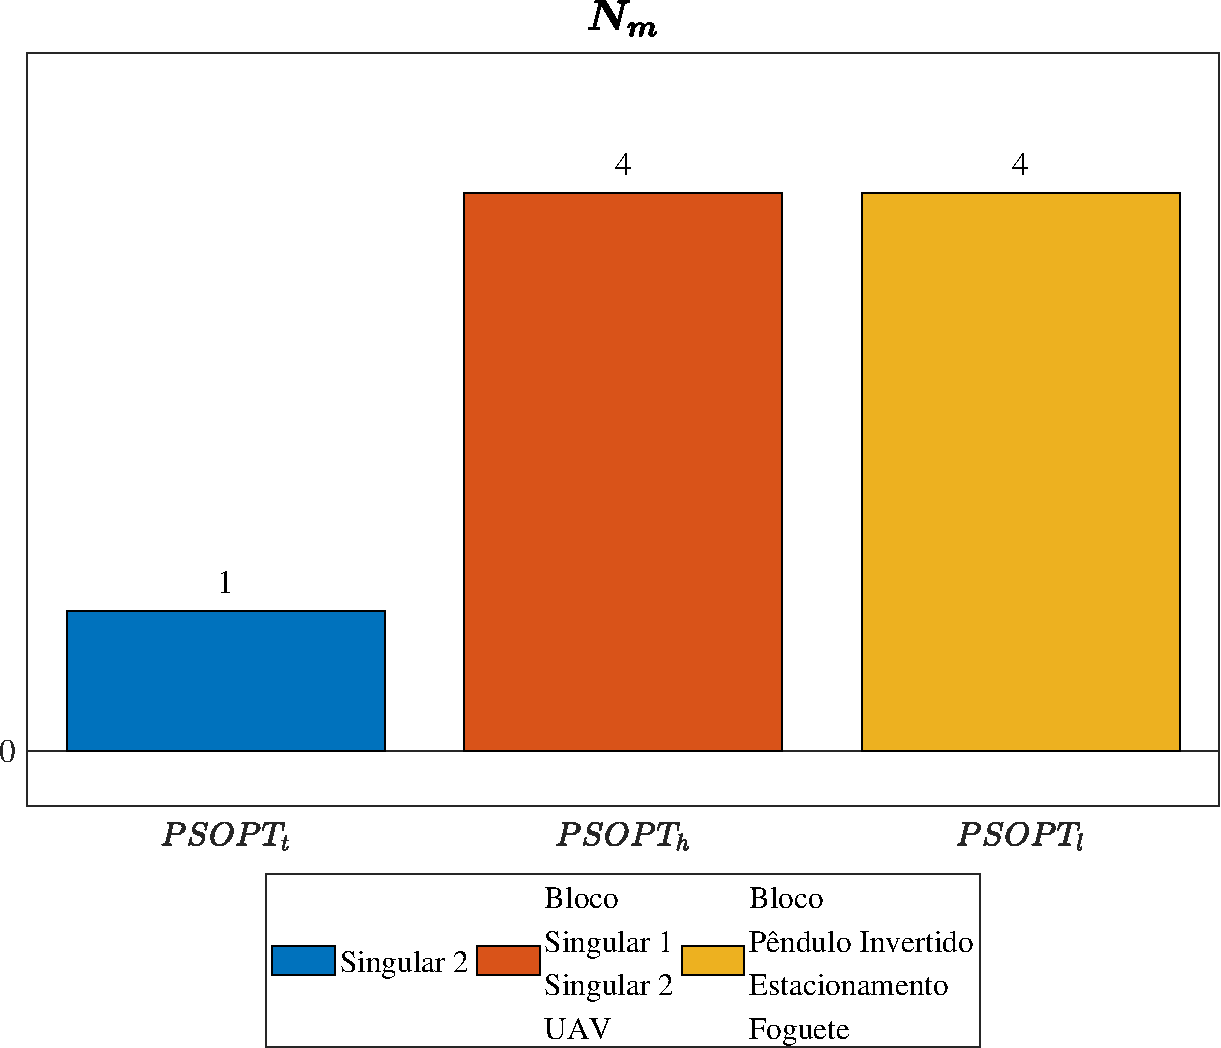
\includegraphics[width=1\linewidth]{fig/resultados/ranking/3/N}
	\captionof{figure}[Avaliação do número de nós de colocação atribuídos ao $ PSOPT_t $, ao $ PSOPT_h $ e ao $ PSOPT_l $]{Avaliação dos $ N_m $ atribuídos ao $ PSOPT_t $, ao $ PSOPT_h $ e ao $ PSOPT_l $.}
	\label{fig:resultados:conclusao:NPSOPTthl}
	\vspace{\onelineskip}
\end{minipage}

Como consequência das diferenças entre os $ N_m $ associados a cada tipo de colocação, verifica-se que, no geral, atribuem-se ao $ PSOPT_l $ e ao $ PSOPT_h $ $ t_p $ menores que os atribuídos ao $ PSOPT_t $, como indica o gráfico apresentado na Figura \ref{fig:resultados:conclusao:tpPSOPTthl}. 

\noindent	
\begin{minipage}{\textwidth}
	\vspace{\onelineskip}
	\centering
	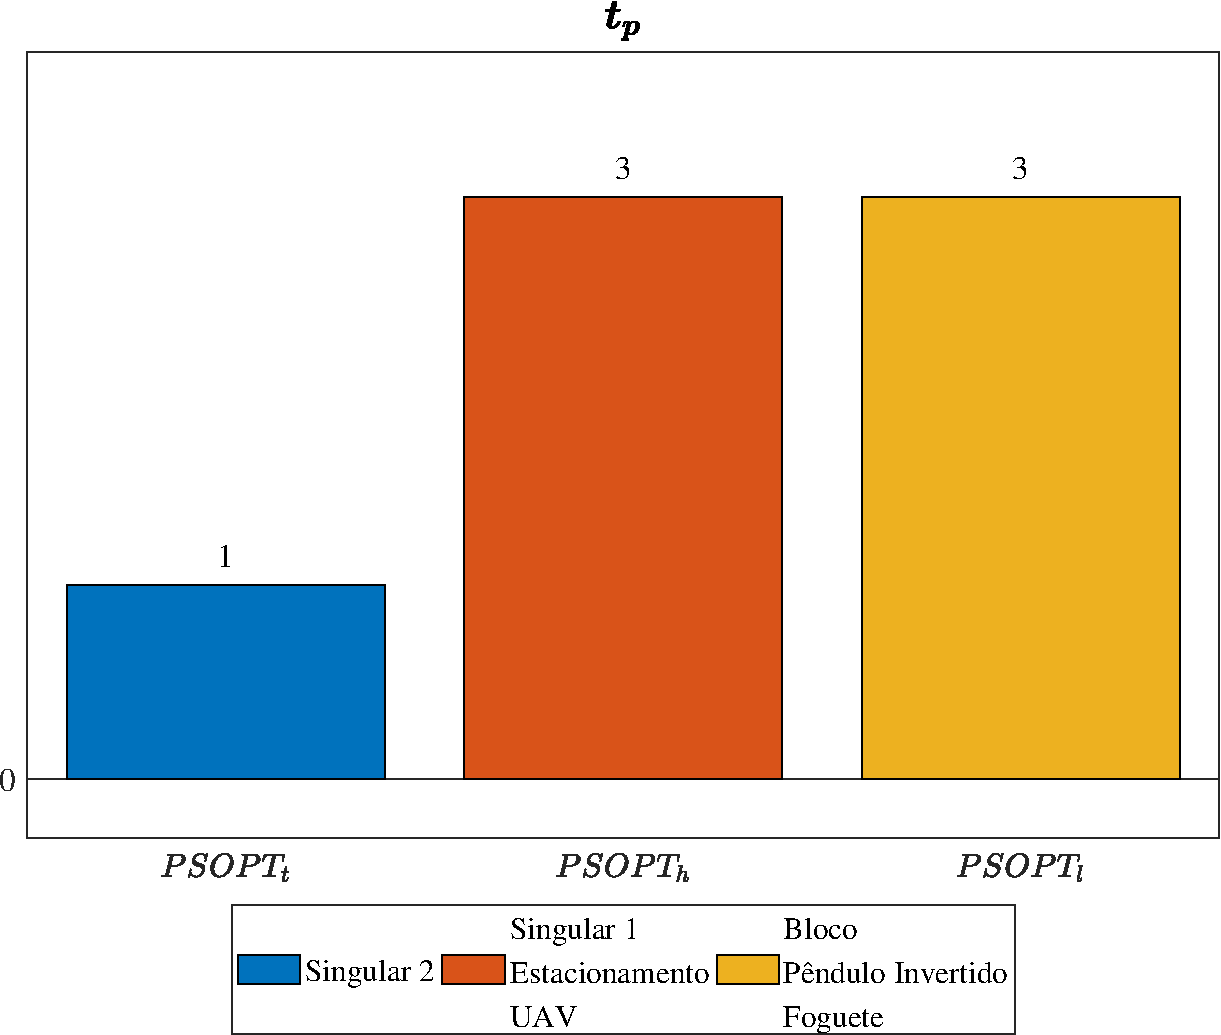
\includegraphics[width=1\linewidth]{fig/resultados/ranking/3/t}
	\captionof{figure}[Avaliação dos tempos de processamento atribuídos ao $ PSOPT_t $, ao $ PSOPT_h $ e ao $ PSOPT_l $]{Avaliação dos $ t_p $ atribuídos ao $ PSOPT_t $, ao $ PSOPT_h $ e ao $ PSOPT_l $.}
	\label{fig:resultados:conclusao:tpPSOPTthl}
	\vspace{\onelineskip}
\end{minipage}

Além disso, estão associados ao $ PSOPT_l $ $ n_{aval} $ menores que os atribuídos ao $ PSOPT_t $ e ao $ PSOPT_h $, como indica o gráfico da Figura \ref{fig:resultados:conclusao:navalPSOPTthl}. Essa máxima vale para a maioria dos estudos de caso monofásicos, com exceção daquele introduzido na Seção \ref{sec:resultados:uav}, no qual verificou-se o distúrbio numérico citado anteriormente. Vale ressaltar que, avaliando-se os resultados introduzidos na Seção \ref{sec:resultados:singulares}, verifica-se que é atribuído ao $ PSOPT_l $ um $ n_{aval} $ menor que os associados ao $ PSOPT_t $ e ao $ PSOPT_h $, ainda que os $ N_m $ atribuídos aos mesmos sejam consideravelmente menores que aquele associado ao $ PSOPT_l $.

\noindent	
\begin{minipage}{\textwidth}
	\vspace{\onelineskip}
	\centering
	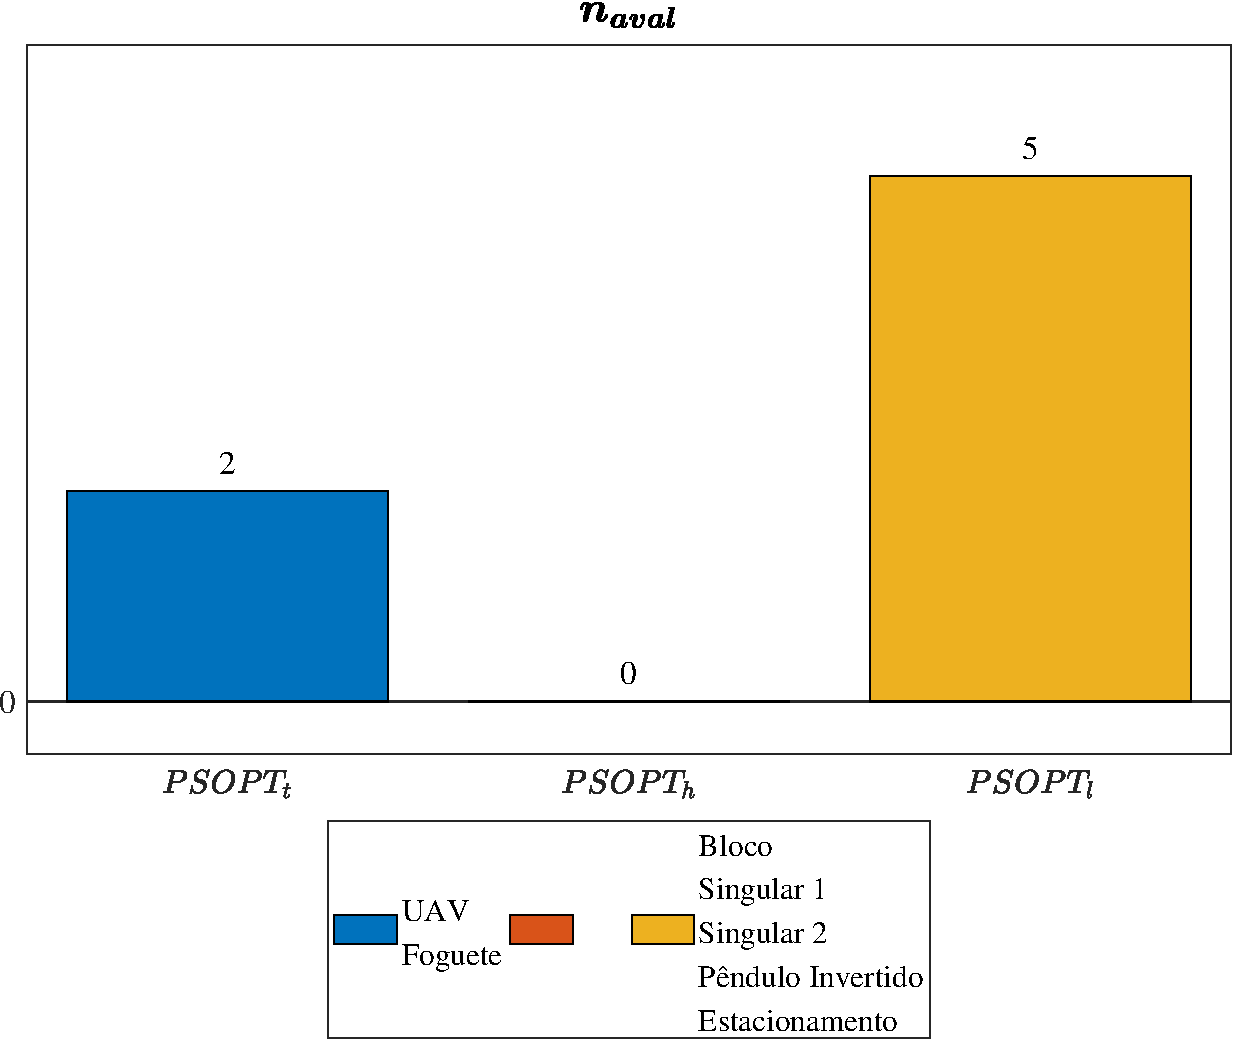
\includegraphics[width=1\linewidth]{fig/resultados/ranking/3/eval}
	\captionof{figure}[Análise do número de avaliações da função objetivo atribuídos ao $ PSOPT_t $, ao $ PSOPT_h $ e ao $ PSOPT_l $]{Avaliação dos $ n_{aval} $ atribuídos ao $ PSOPT_t $, ao $ PSOPT_h $ e ao $ PSOPT_l $.}
	\label{fig:resultados:conclusao:navalPSOPTthl}
	\vspace{\onelineskip}
\end{minipage}

Comparando-se ainda as soluções obtidos por meio do $ PSOPT_t $, do $ PSOPT_h $, do $ COPILOTS_t $, e do $ COPILOTS_h $, observa-se que os $ N_m $ associados à colocação Hermite-Simpson são tipicamente menores que aqueles atribuídos à colocação trapezoidal, como indicam os gráficos apresentados nas Figuras \ref{fig:resultados:conclusao:NthCOPILOTS} e \ref{fig:resultados:conclusao:NthPSOPT}. Esses resultados se devem às propriedades numéricas inerentes a cada tipo de colocação e dos métodos empregados na interpolação dos estados e controles.

\noindent	
\begin{minipage}{\textwidth}
	\vspace{\onelineskip}
	\centering
	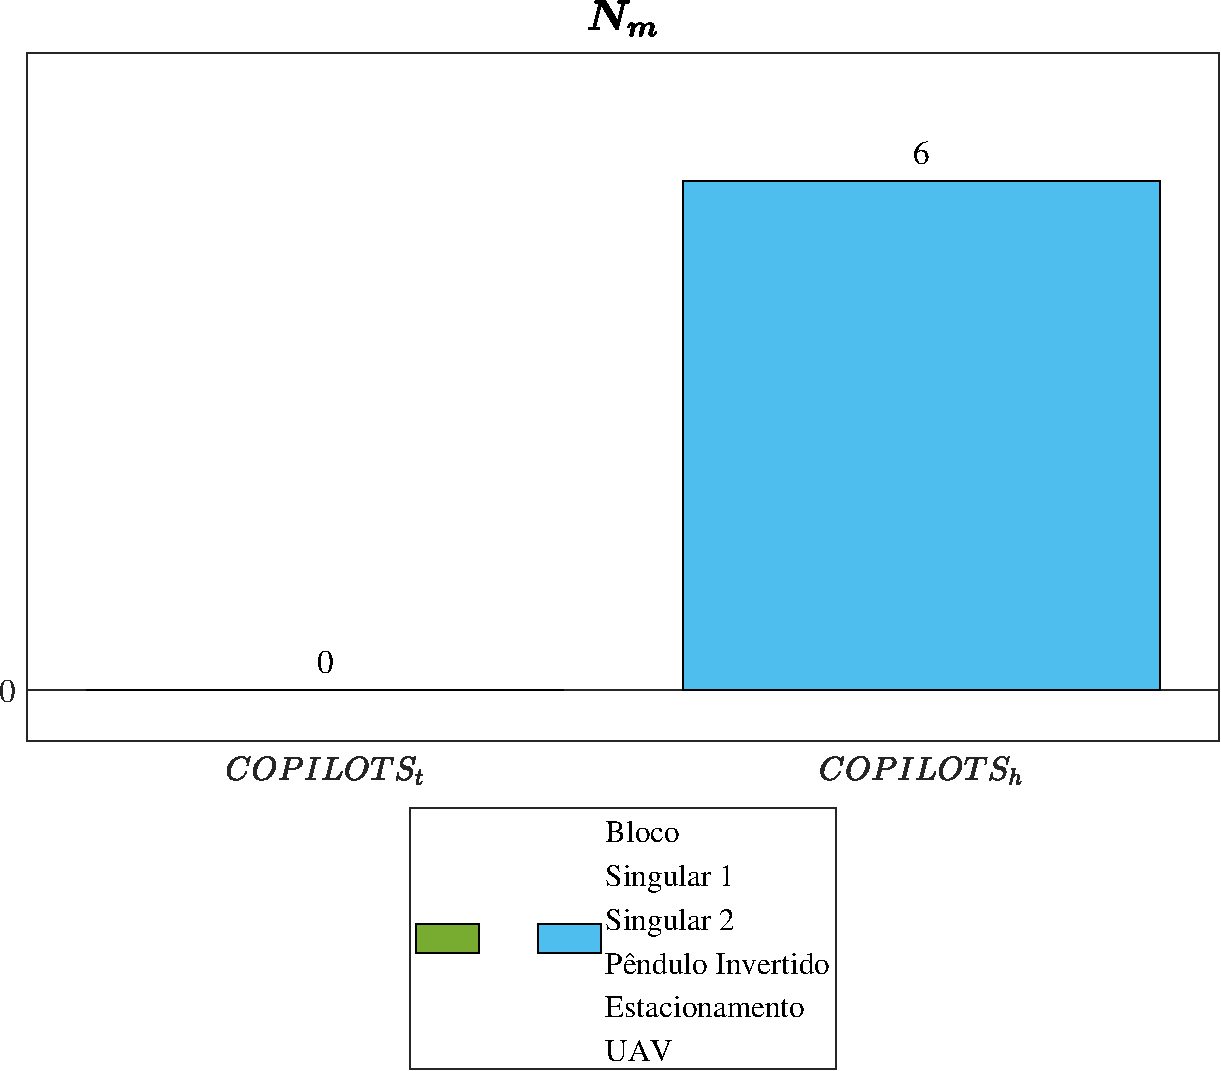
\includegraphics[width=1\linewidth]{fig/resultados/ranking/2/N}
	\captionof{figure}[Avaliação do número de nós de colocação atribuídos ao $ COPILOTS_t $ e ao $ COPILOTS_h $]{Avaliação dos $ N_m $ atribuídos ao $ COPILOTS_t $ e ao $ COPILOTS_h $.}
	\label{fig:resultados:conclusao:NthCOPILOTS}
	\vspace{\onelineskip}
\end{minipage}

\noindent	
\begin{minipage}{\textwidth}
	\vspace{\onelineskip}
	\centering
	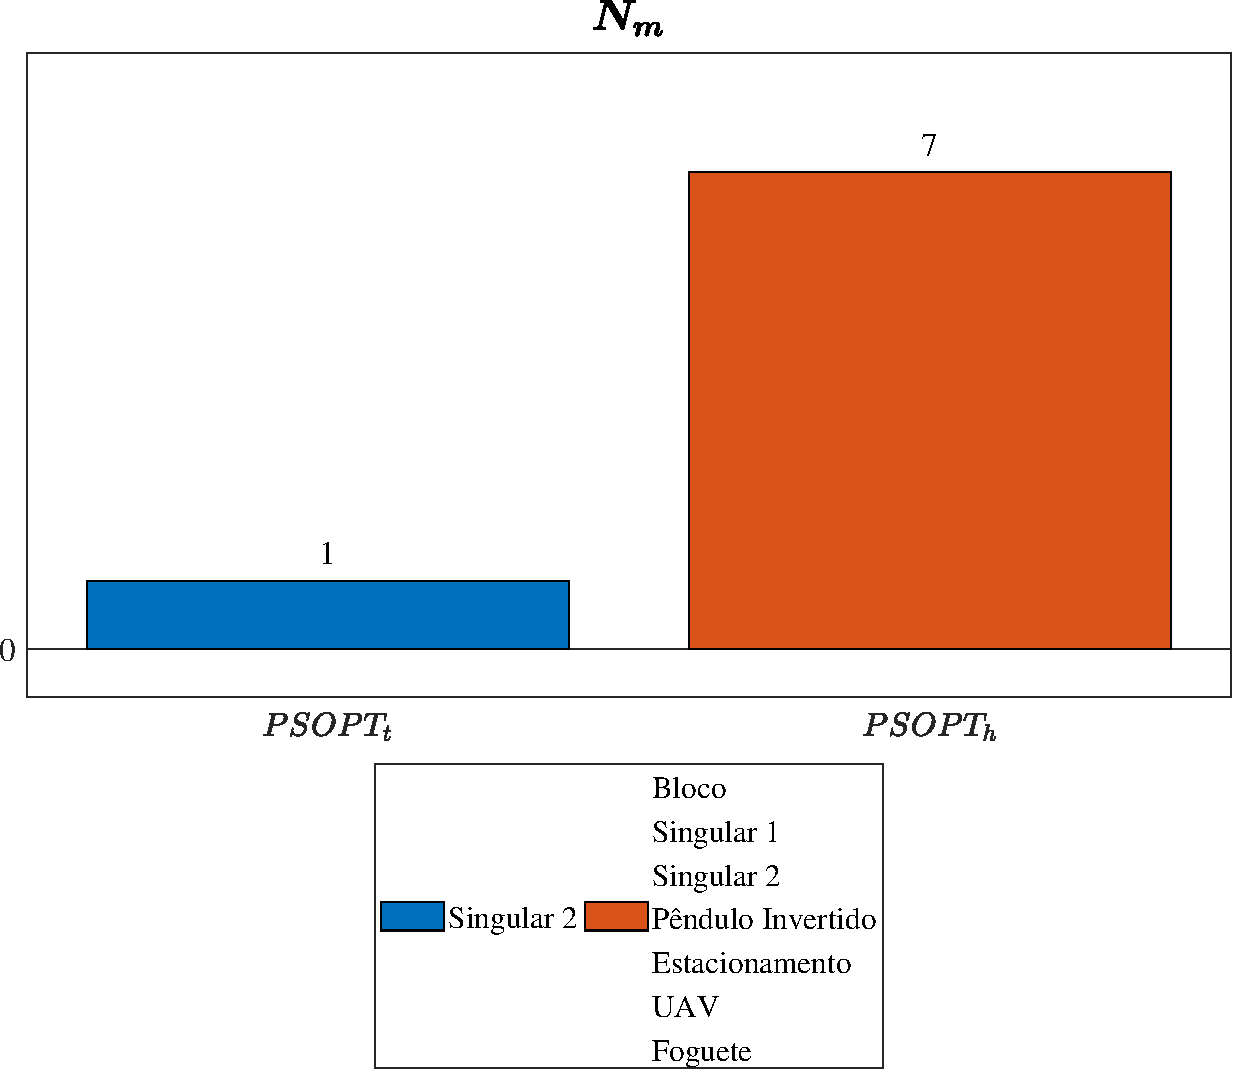
\includegraphics[width=1\linewidth]{fig/resultados/ranking/1/N}
	\captionof{figure}[Avaliação do número de nós de colocação atribuídos ao $ PSOPT_t $ e ao $ PSOPT_h $]{Avaliação dos $ N_m $ atribuídos ao $ PSOPT_t $ e ao $ PSOPT_h $.}
	\label{fig:resultados:conclusao:NthPSOPT}
	\vspace{\onelineskip}
\end{minipage}

\todo[inline, color=pink, size=normalsize]{Problemas singulares no $ PSOPT $}

Como esperado, verifica-se que o emprego da colocação pseudo-espectral na solução de PCOs singulares não traz resultados satisfatórios \cite{becerra_tutorial_2010}. De fato, nas soluções atribuídas ao $ PSOPT_l $, introduzidas na Seção \ref{sec:resultados:singulares}, observam-se $ N_m $ bastante altos e trajetórias de controle consideravelmente oscilatórias. Resultados mais aceitáveis poderiam ser obtidos caso os PCOs singulares fossem formulados empregando-se múltiplas fases \cite{nascentes_resolucao_2012}. Uma outra alternativa seria empregar a abordagem introduzida na Seção \ref{sec:resultados:conclusao:suavizacaoTrajetorias}, que possibilita a obtenção de trajetórias mais suaves.

\todo[inline, color=pink, size=normalsize]{Limitação do Método de Ponto Interior do $ PSOPT $}

Além disso, verifica-se que o Método de Ponto Interior no qual se baseia o IPOPT \cite{wachter_implementation_2006}, pacote utilizado pelo $ PSOPT $ na solução de PPNLs, não apresenta um bom desempenho quando empregado na resolução de PCOs que contenham muitas restrições em sua formulação. De fato, avaliando-se os resultados apresentados na Tabela \ref{tab:estacionamento:raw}, nota-se que são atribuídos ao $ PSOPT $ $ N_s\% $ consideravelmente baixos. 

\todo[inline, color=pink, size=normalsize]{Trajetórias do $ PSOPT_l $}

Verifica-se que as trajetórias construídas com base nos resultados advindos da colocação pseudo-espectral são consideravelmente mais suaves que aquelas produzidas por meio de outros tipos de colocação. Esse comportamento se deve ao fato das trajetórias associadas à colocação pseudo-espectral serem interpoladas globalmente, empregando-se um único polinômio de alta ordem \cite{becerra_psopt_2019}. 

\todo[inline, color=pink, size=normalsize]{Reconstrução da trajetória do $ PSOPT_h $:}

É essencial frisar que os dados fornecidos pelo $ PSOPT_h $, após a resolução de um estudo de caso qualquer, são insuficientes para que construam-se as trajetórias de controle. Isso porque a interpolação de trajetórias na qual se baseia a colocação Hermite-Simpson depende não só dos valores que $ \mathbf{u}(t) $ assume nos nós de colocação, mas também dos valores assumidos por $ \mathbf{u}(t) $ nos nós intermediários, que não são fornecidos pelo $ PSOPT $. 

\todo[inline, color=pink, size=normalsize]{Qualidades do $ FALCON $}

Verifica-se que na maioria dos casos são atribuídos ao $ FALCON $ os menores $ t_p $ e $ n_{aval} $, como indicam os gráficos nas Figuras \ref{fig:resultados:conclusao:tpFALCON} e \ref{fig:resultados:conclusao:navalFALCON}. Além disso, normalmente estão associados a esse pacote $ N_s\% $ bem próximos a 100\%. Esses resultados podem ser justificados por dois principais fatores. Primeiro, ao uso que o $ FALCON $ faz de ferramentas simbólicas na obtenção das derivadas analíticas da função objetivo e das restrições, e segundo, à geração e ao emprego de arquivos de extensão \texttt{.mex}, que convertem, de forma automática, os códigos em Matlab\textsuperscript{\textregistered} utilizados na formulação do PCO em rotinas baseadas em linguagens de baixo nível como C/C++ e Fortran. De fato, é sabido que o emprego de derivadas analíticas acarreta uma diminuição no número de avaliações da função objetivo e consequentemente no tempo de processamento \cite{betts_practical_2001}. Além disso, o emprego de linguagens de baixo nível pré-compiladas proporciona uma redução ainda maior no tempo de processamento \cite{febbo_nloptcontrol_2020}. 

\noindent	
\begin{minipage}{\textwidth}
	\vspace{\onelineskip}
	\centering
	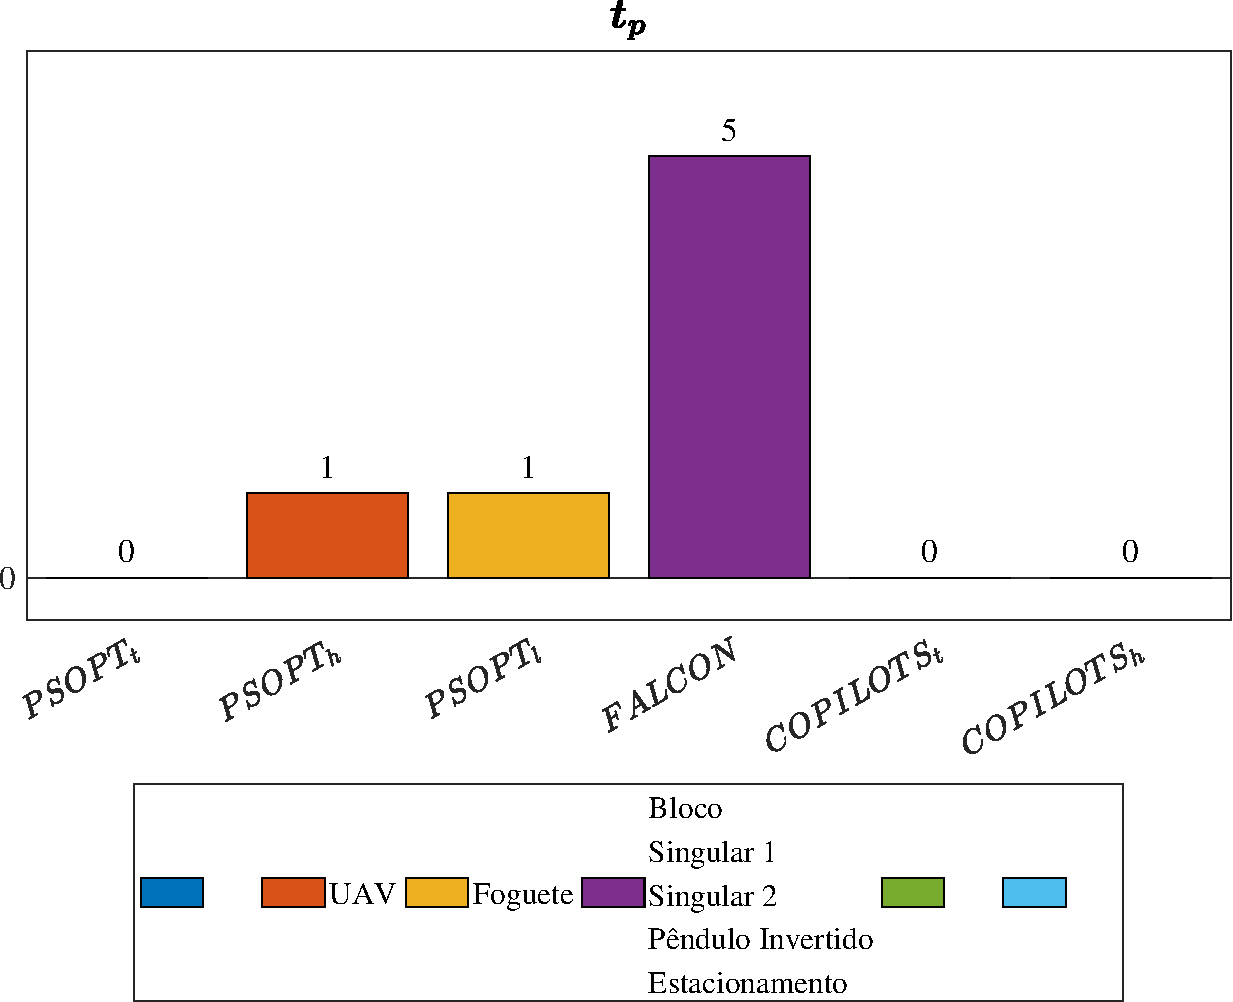
\includegraphics[width=1\linewidth]{fig/resultados/ranking/all/t}
	\captionof{figure}[Avaliação dos tempos de processamento atribuídos a todos os pacotes avaliados]{Avaliação dos $t_p$ atribuídos a todos os pacotes avaliados.}
	\label{fig:resultados:conclusao:tpFALCON}
	\vspace{\onelineskip}
\end{minipage}

\noindent	
\begin{minipage}{\textwidth}
	\vspace{\onelineskip}
	\centering
	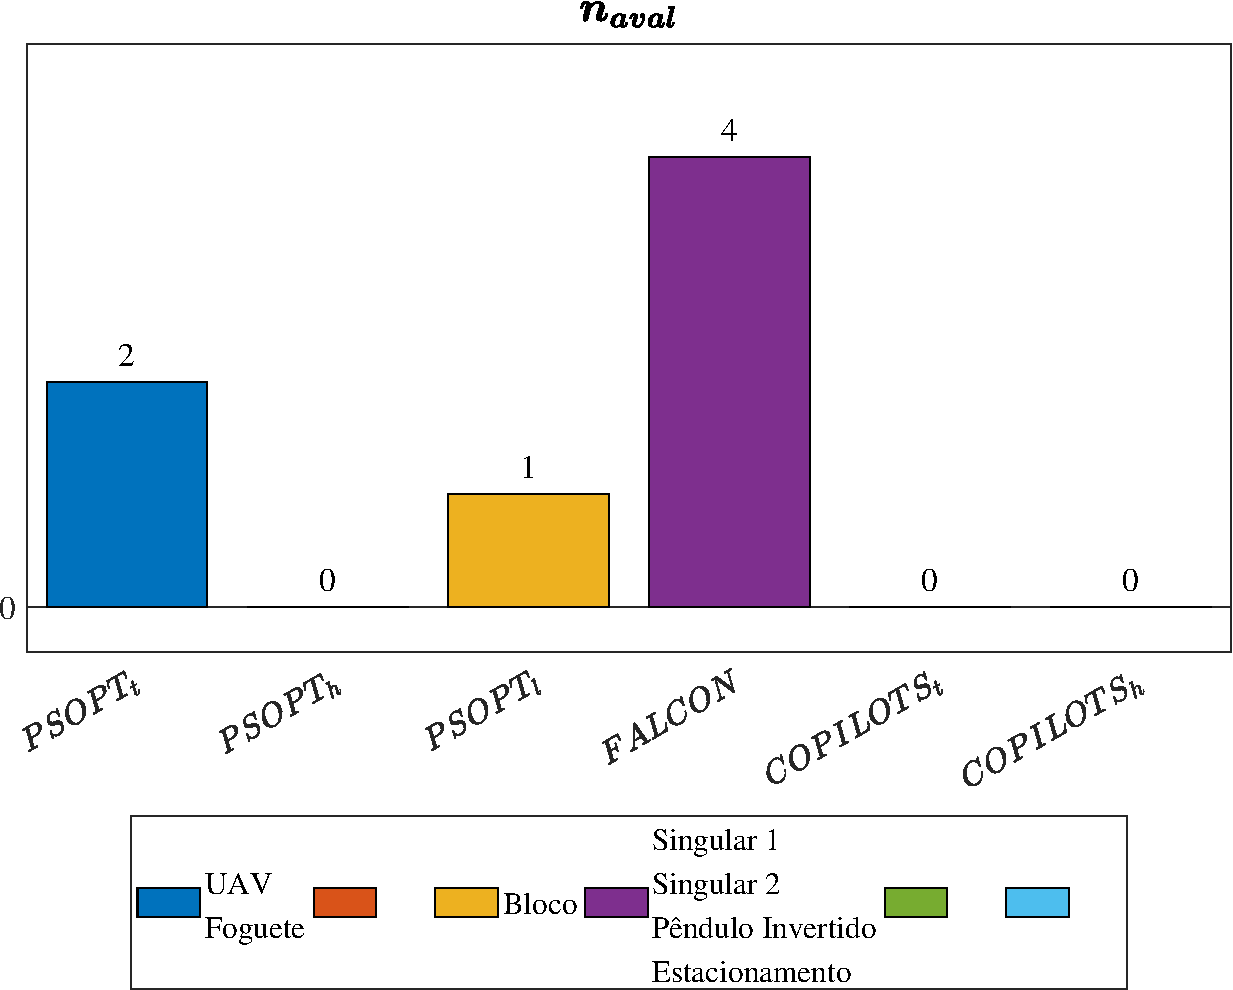
\includegraphics[width=1\linewidth]{fig/resultados/ranking/all/eval}
	\captionof{figure}[Análise do número de avaliações da função objetivo atribuídas a todos os pacotes avaliados]{Avaliação dos $ n_{aval} $ atribuídos a todos os pacotes avaliados.}
	\label{fig:resultados:conclusao:navalFALCON}
	\vspace{\onelineskip}
\end{minipage}

Destaca-se que o único estudo de caso, formulado com base em uma única fase, no qual não é atribuído ao $ FALCON $ o menor $ t_p $, é aquele apresentado na Seção \ref{sec:resultados:uav}. Esse resultado indica que e pacote tem, de fato, como principal vantagem a computação de derivadas analíticas, recurso que não pode ser empregado no estudo de caso em questão, uma vez que a dinâmica associada ao mesmo depende da interpolação linear dos dados de uma tabela. 

\todo[inline, color=pink, size=normalsize]{$ FALCON $ e o impacto de $ N $}

Além do mais, verifica-se que os $ t_p $ e $ n_{aval} $ associados ao $ FALCON $ são praticamente insensíveis ao aumento de $ N $, devido ao uso que esse pacote faz de ferramentas simbólicas na computação de derivadas analíticas. Nas Figuras \ref{fig:resultados:conclusao:Nxt} e \ref{fig:resultados:conclusao:Nxn}, que têm o eixo das abcissas em escala logarítmica, são comparados os $ t_p $ e $ n_{aval} $ associados à resolução do estudo de caso introduzido na Seção \ref{sec:resultados:penduloInvertido}, empregando-se o $ PSOPT_t $ e o $ FALCON $, e considerando-se $ N $ razoavelmente altos. Por meio da avaliação desses resultados, é possível verificar primeiramente que, para $ N $ pequenos, o $ FALCON $ executa tão rapidamente quando o $ PSOPT_t $, que é baseado nas linguagens C/C++, e que os $ t_p $ associados ao primeiro, diferentemente daqueles atribuídos ao segundo, são muito pouco sensíveis ao aumento de $ N $. 

Vale ressaltar, no entanto, que essa diferença nos $ t_p $ associados ao $ FALCON $ e ao $ PSOPT $ se devem principalmente ao cálculo do erro de discretização das equações diferenciais associadas à dinâmica do PCO, computado pelo $ PSOPT $ mas não pelo $ FALCON $. O tempo gasto no processamento desse erro aumenta consideravelmente à medida que $ N $ cresce, enquanto o tempo despendido de fato na solução do PPNL não apresenta um crescimento considerável à medida que $ N $ aumenta.  

Além disso, é possível verificar que os $ n_{aval} $ associados ao $ FALCON $ são significativamente menores que os atribuídos ao $ PSOPT_t $, e praticamente insensíveis ao aumento de $ N $. Esse resultado se deve ao uso que o $ FALCON $ faz das derivadas analíticas da função objetivo e das restrições. 

\noindent	
\begin{minipage}{\textwidth}
	\vspace{\onelineskip}
	\centering
	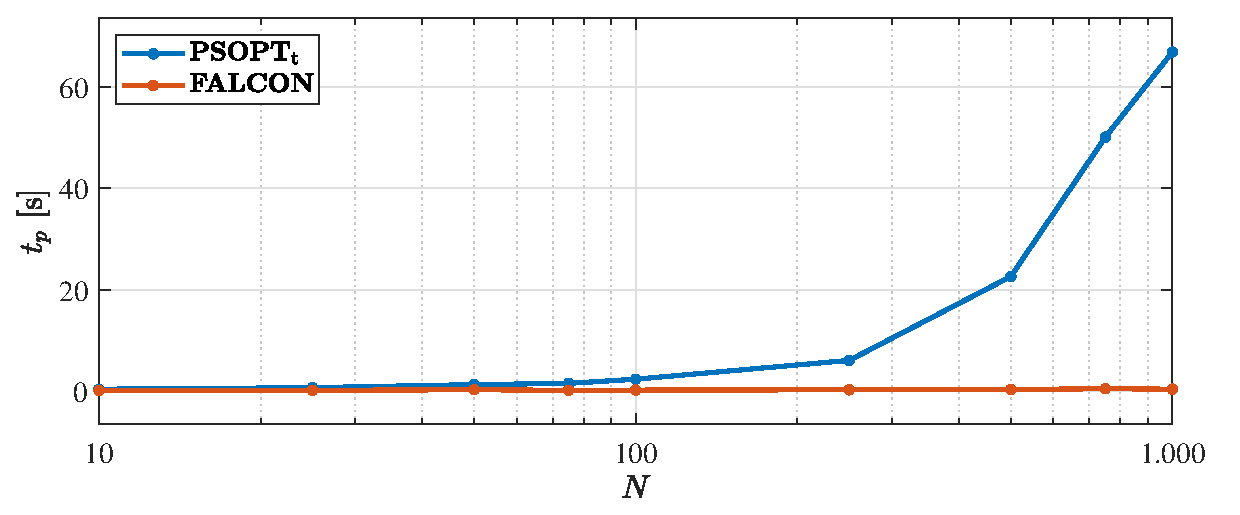
\includegraphics[width=1\linewidth]{fig/resultados/obs/bigN/Nxt}
	\captionof{figure}[Avaliação dos tempos de processamentos atribuídos ao $ PSOPT_t $ e o $ FALCON $, para o problema do pêndulo invertido, considerando-se um número de nós de colocação razoavelmente alto]{Comparação entre os $ t_p $ associados à resolução do estudo de caso apresentado na Seção \ref{sec:resultados:penduloInvertido} empregando-se o $ PSOPT_t $ e o $ FALCON $, e considerando-se $ N $ razoavelmente altos.}
	\label{fig:resultados:conclusao:Nxt}
	\vspace{\onelineskip}
\end{minipage}

\noindent	
\begin{minipage}{\textwidth}
	\vspace{\onelineskip}
	\centering
	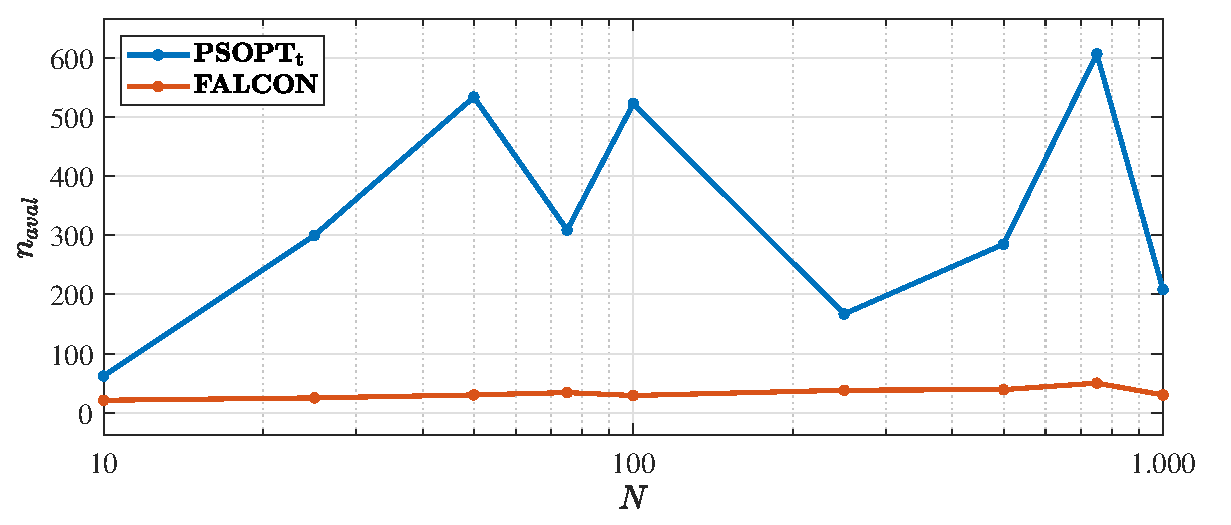
\includegraphics[width=1\linewidth]{fig/resultados/obs/bigN/Nxn}
	\captionof{figure}[Análise das avaliações da função objetivo atribuídas ao $ PSOPT_t $ e o $ FALCON $, para o problema do pêndulo invertido, considerando-se um número de nós de colocação razoavelmente alto]{Comparação entre os $ n_{aval} $ associados à resolução do estudo de caso apresentado na Seção \ref{sec:resultados:penduloInvertido} empregando-se o $ PSOPT_t $ e o $ FALCON $, e considerando-se $ N $ razoavelmente altos.}
	\label{fig:resultados:conclusao:Nxn}
	\vspace{\onelineskip}
\end{minipage}

\todo[inline, color=pink, size=normalsize]{$ FALCON $ e os multifásicos}

Apesar dos bons resultados obtidos por meio do $ FALCON $, é preciso ressaltar que o estudo de caso introduzido na Seção \ref{sec:resultados:foguete} não pode ser resolvido pelo emprego desse pacote, já que, nesse caso, o processo de otimização atinge um mínimo local que não atende às restrições do problema e ali permanece. O PCO associado a esse estudo de caso possui múltiplas fases e, apesar do $ FALCON $ ser capaz de resolver problemas desse tipo, não é apresentada na documentação associada a esse pacote qualquer exemplo de um problema multifásico que tenha dinâmicas distintas associadas a cada fase, como é o caso do PCO em questão. 

\todo[inline, color=pink, size=normalsize]{Observações sobre o $ COPILOTS $}

Verifica-se que ao $ COPILOTS $ estão comumente atribuídos os menores $ J^* $, como indica o gráfico na Figura \ref{fig:resultados:conclusao:JCOPILOTS}, e os maiores $ N_s\% $, devido ao uso que o pacote faz do SQP. Em contrapartida, ao $ COPILOTS $ estão também associados os maiores $ t_p $ e $ n_{aval} $, não só pelo emprego do $ SQP $, mas também devido ao uso que o $ COPILOTS $ faz da função \texttt{fmincon()}, nativa do Matlab\textsuperscript{\textregistered}, na solução de PPNLs, algo que é fortemente desaconselhado pelos desenvolvedores de outros pacotes \cite{falugi_iclocs2_2018}. O uso dessa função pode inclusive explicar os baixíssimos $ N_s\% $ atribuídos ao $ COPILOTS $ na resolução dos estudos de caso introduzidos nas Seções \ref{sec:resultados:estacionamento}, que apresenta um número consideravelmente alto de restrições, e \ref{sec:resultados:uav}, que possui uma dinâmica descontínua que depende da interpolação linear dos dados de uma tabela. Além disso, verifica-se que os menores $ J^* $ são atribuídos aos métodos que fazem uso da colocação Hermite-Simpson, devido às propriedades numéricas associadas a esse tipo de colocação, que faz uso de nós intermediários na interpolação dos estados e controles. 

\noindent	
\begin{minipage}{\textwidth}
	\vspace{\onelineskip}
	\centering
	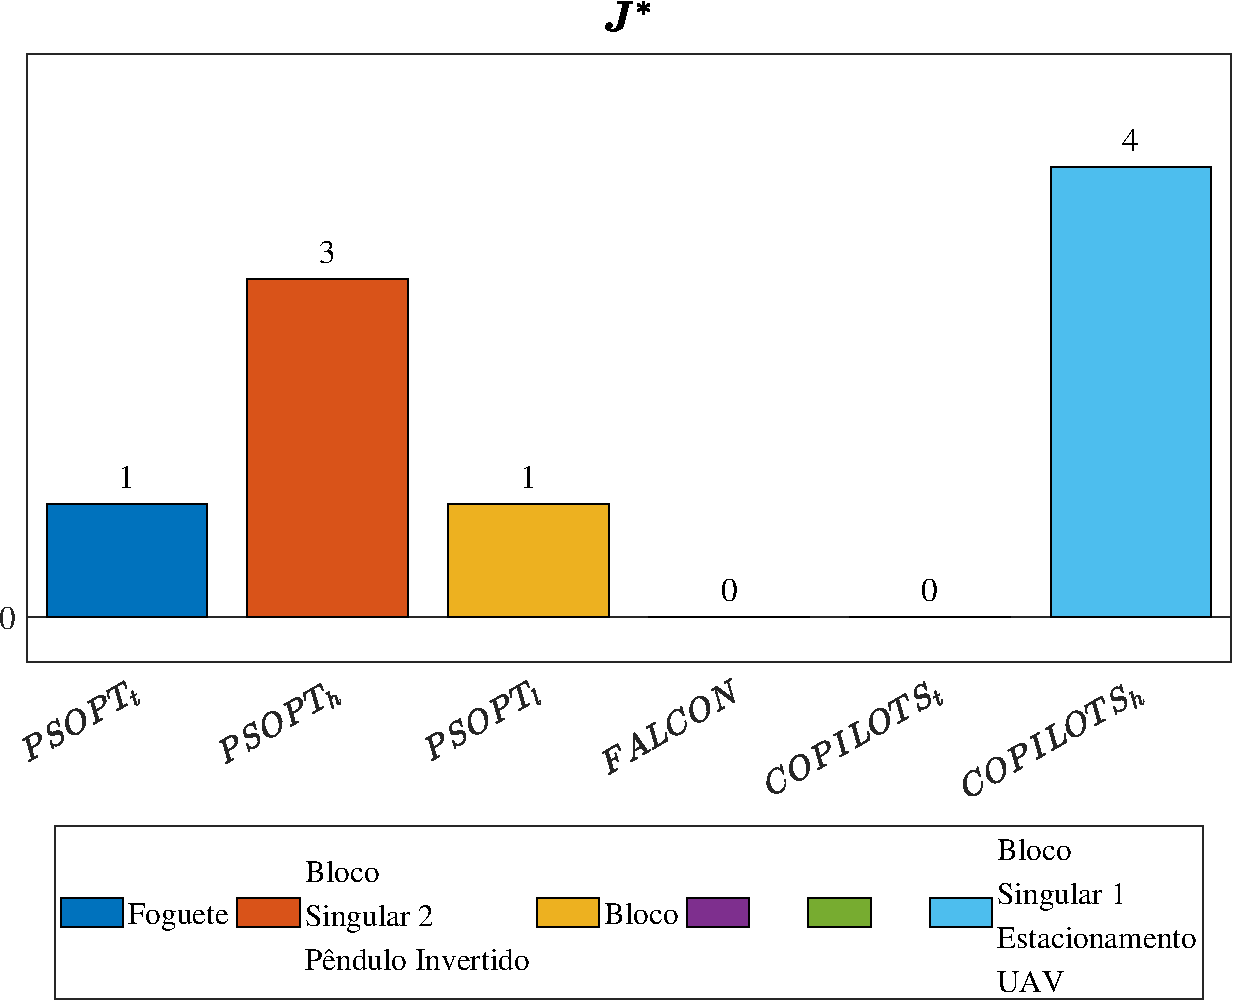
\includegraphics[width=1\linewidth]{fig/resultados/ranking/all/J}
	\captionof{figure}[Avaliação dos valores ótimos da função objetivo atribuídos a todos os pacotes avaliados]{Avaliação dos $ J^* $ atribuídos a todos os pacotes avaliados.}
	\label{fig:resultados:conclusao:JCOPILOTS}
	\vspace{\onelineskip}
\end{minipage}

\todo[inline, color=pink, size=normalsize]{Resumo}

Os resultados obtidos podem ser resumidos da seguinte forma:
\begin{itemize}
	\item Recomenda-se o emprego do $ PSOPT $ na resolução de PCOs multifásicos;
	\item Não é recomendado que a colocação pseudo-espectral seja empregada na resolução de PCOs singulares;
	\item No caso em que a minimização da função objetivo é especialmente relevante e que o tempo de execução, assim como o número de avaliações da função objetivo, são pouco importantes, recomenda-se que o $ COPILOTS $ seja utilizado juntamente à colocação Hermite-Simpson;
	\item Caso o usuário tenha pouca ou nenhuma experiência com a implementação computacional de PCOs, ou caso tenha o intuito empregar um pacote computacional para fins didáticos, recomenda-se a utilização do $ COPILOTS $;
	\item Caso seja necessário resolver um PCO empregando o mínimo de avaliações da função objetivo no menor tempo possível, recomenda-se o emprego do $ FALCON $;
	\item Não é recomendado que o $ FALCON $ seja utilizado na resolução de PCOs multifásicos que possuam uma dinâmica distinta associada a cada fase;
\end{itemize}